%!TEX root = ../crimson_throne_book_main.tex
% 2014-10-04
The\hyperref[fig:Carowyn-villa-486295633]{ Carowyn home } is a stately manor along Shoreline Way, just a street away from the companions' own villa. It serves as the in-town house of Ausio and Olauren Carowyn, a small noble family with lots of land outside the city, where lord Carowyn prefers to spend most of his days. His son, Cedrik, however, is more inclined to stay in the city, officially to look over his family's interests, but his main reasons are of a personal nature. Like most young men he enjoys the excitement of city-life. Since his family's city estate is actually built for entertaining, Cedrik takes full advantage of that by regularly throwing parties for his peers as a way to raise his house's standing among the older noble families. When the companions arrive at his Bloodsworn mahogany front door, he welcomes them with open arms. Had he known that the heroes of the city were interested in coming to his masquerade party, he would have invited them himself, he claims. He shows his guest into the great hall, where Ruan Mirukova from the Marble Dome's orchestra is playing some music and his sister Deyanira is dancing. A scantily-clad woman serves the newcomers a drink, as they politely say hello to the visitors in this room. Valdur Bromathan V makes for a far less impressive barbarian in his Shoanti outfit than Balian in his rattlebone armor, while Derrik Jeggare, lord Mercival's son, is dressed as a lion and Alice Fordyce makes for a fearsome pirate. The cutest person in this hall is doe-eyed shepherdess Siri Leroung. \\

\begin{figure}[h]
	\centering
	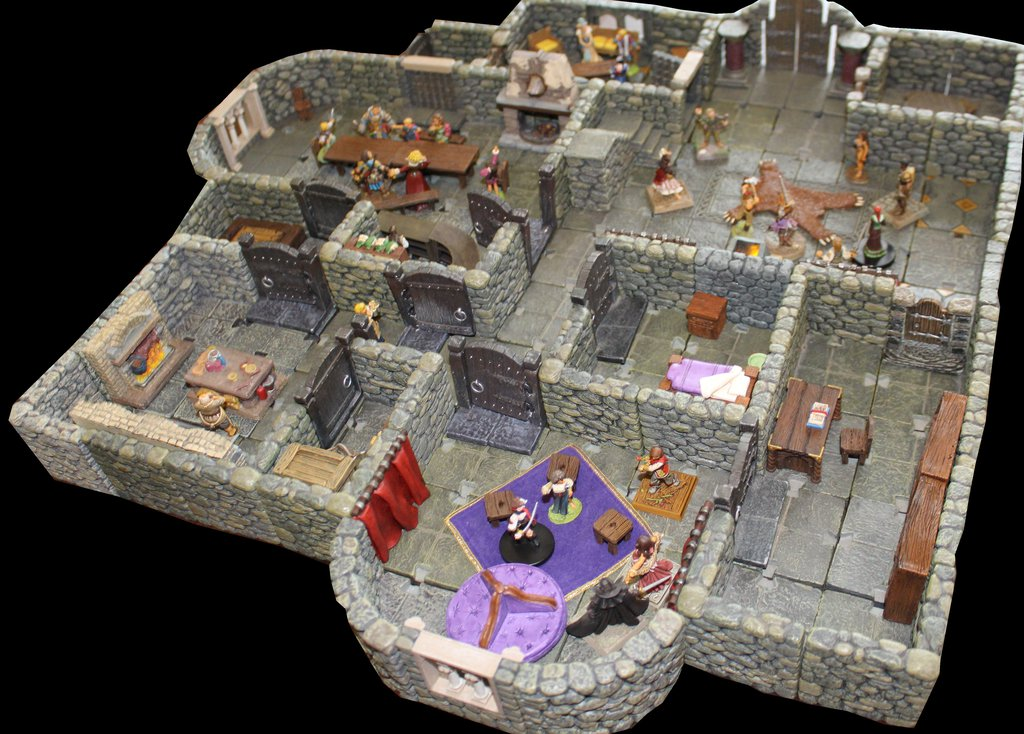
\includegraphics[width=0.39\textwidth]{images/Carowyn-villa-486295633.jpg}
	\caption{Carowyn villa}
	\label{fig:Carowyn-villa-486295633}
\end{figure}

In the front sitting room the companions reconnect with Aaron Endrin, the eldest son of Marcus Endrin, the commander of the Sable Company. Aaron has started his training to become a Sable marine himself, after serving his father as a squire for many years. This role is now being observed by his smaller brother, Jonas, who is here as well. Quint remembers seeing Aaron with Marguerite Jeggare at the grand feast in her family's museum three weeks ago, so he informs if Korvosa's most beautiful girl is here as well. Aaron tells him she won't be attending parties any time soon, as she has joined the queen's guard to serve as one of the Grey Maidens. Quint is quite surprised to hear that, but Aaron explains that he understands the call of military duty. Despite her beauty Marguerite is not an air-headed puppet, but a self-confident and principled young lady who is allowed to make her own choices in life. Christina Leroung disapproves of Marguerite's "dumb" decision. She can understand Aaron's ambition to join the Sable Company, as he was born to become their next commander, but she cannot get why someone from a noble family would chose to play the part of an anonymous soldier, certainly not if she has Marguerite's looks. That girl can get any man she wants, so why she prefers to waste her time chasing windmills is beyond Christina. While the conversation is on the topic of the Grey Maidens, Quint also asks Aaron if he knows where all those new soldiers suddenly came from. Aaron confirms that one ship was registered coming from Cheliax with over a hundred Maiden recruits. Neither the Leroungs nor the Endrins have any sick family members at the moment, although they do realize the threat: diseases do not stop at a nobleman's door.\\

In the dining hall the companions come across even more guests. Verana Ornelos is trying her best to hide her average features by dressing up as a hot succubus, succeeding only partially at the job. Her younger sister Julia possesses a lot more natural grace and looks stunning as a fairy princess. The cute little noble lacks her family's knack for magic, however, so she will be one of the few Ornelos children not pursuing a career in spell-weaving. Her sister Verana, on the other hand, will shortly start her Acadamae education. Belinda Zenderholm takes some time to get to know the companions better. She has heard many good things about them from her mother, high judge Zenobia. She cautions Sjo not to encourage Amin Jalento to drink too much. He is rumored to have got really drunk at the Riverwind Festival three days ago, spoiling what is left of his reputation and his family's good name by whoring and drinking in Eel's End. He is already quite inebriated and shows no signs of slowing down. He wants to share a drink with the men who saved him from half a dozen hot-tempered dockworkers during the riots. He is also glad his father, the "respectable" captain, is not here to rebuke him some more, as he is prone to do, preferably in public. Another person in this room is Perishial Kalissreavil, the half-elven ambassador of the Mierani Elves. He totally lives up to his reputation of womanizer by flirting with Julia Ornelos. Before long he smooth talks her into following him upstairs.\\

The companions meet their closest friends among the city's nobles in the music room. Aisha Leroung, the star of the Saint Alika opera, makes for a sexy vampire tonight. She immediately clings to Quint's arm and wants to know what he's been up to. She has not started a new project herself yet, but she hopes the Marble Dome's director Touran Palastus comes up with something soon. Flamboyant Xerxes Jeggare has chosen to come as Blackjack and feels inspired to play some music with Sjo, Quint and Puk. He takes a seat behind the harpsichord and starts a little session that draws more guest to the back room. His sister Maud is as fine company as ever, joking and laughing in her pretty peacock dress. Sjo strikes up a conversation with Sara Bromathan, who is dressed up as a chaste version of Sarenrae. Like her father she envisions a career serving the sun goddess. She wonders about the source of Sjo's strange divine powers, as she knows from her father that Sjo served as an acolyte to Sarenrae for some time, but then dropped out. Sjo explains that his powers come to him naturally; he has a special talent for fire magic, which puzzles Sara even more. She thinks it might have been wiser to pursue the same path as Verana Ornelos and train as a wizard, but Sjo figures that his powers are more like those of the Shoanti shamans.(Although Sjo is officially an "oracle", that name does not really fit the bill, so if we call him anything at all, we prefer to use the term "shaman", which has absolutely nothing to do with the new shaman class.) Quint remembers why he and his friends came here, to secretly watch over the guests tonight, so he invites everyone back into the main hall, trying to get as many people together as possible. He cannot avoid that some invitees wander off into the dining room to get something at the bar, but with the open door between the two spaces, he can keep tabs on the people in there as well. While the pleasantries of the evening further unfold, the fire in the hearth suddenly flickers and dies out. The candles in the great chandelier follow one second later, plummeting the room in darkness and startling some of the girls. Sjo, who was standing next to fireplace, has no trouble seeing in the dark. His vision might be limited, but it is also more powerful at short distance, allowing him the gift of darkvision. Realizing that he is probably the only one in the room who can see now, a slight grin slips over his face as he reaches for the wood in the hearth. He sends a {\itshape touch of flame} through his fingers to relight the firewood, but is surprised to see a shadowy creature crawling down from the chimney, just inches from his face. The sighs of surprise from the girls turn to screams of terror now. How could Sjo have missed that thing in the dark? Unless the shadow did not show up in his darkvision ... that must be it! With the fire still licking his fingers, Sjo makes for the creature, but the flames do not seem to hurt it. With his other hand the Shoanti pushes back Sara Bromathan, trying to move her out of harm's way. As the fire on his hand dies out again, the room sinks back into darkness and the creature disappears in the black once more. Balian draws his blade and Puk unsheathes his silver blade, both of them standing ready to react. Then Quint casts a  {\itshape light} spell on one of his devil's horns. Although the brightness of his light seems to suffer from the presence of the shadow, \hyperref[fig:Carowyn-villa-shadow-attack-486296086]{ it does reveal that the creature has already flown out of the fireplace and wrapped its dark tendrils around the servant girl } . The frozen look of death stares from her eyes, as she slips to the floor. \\

\begin{figure}[h]
	\centering
	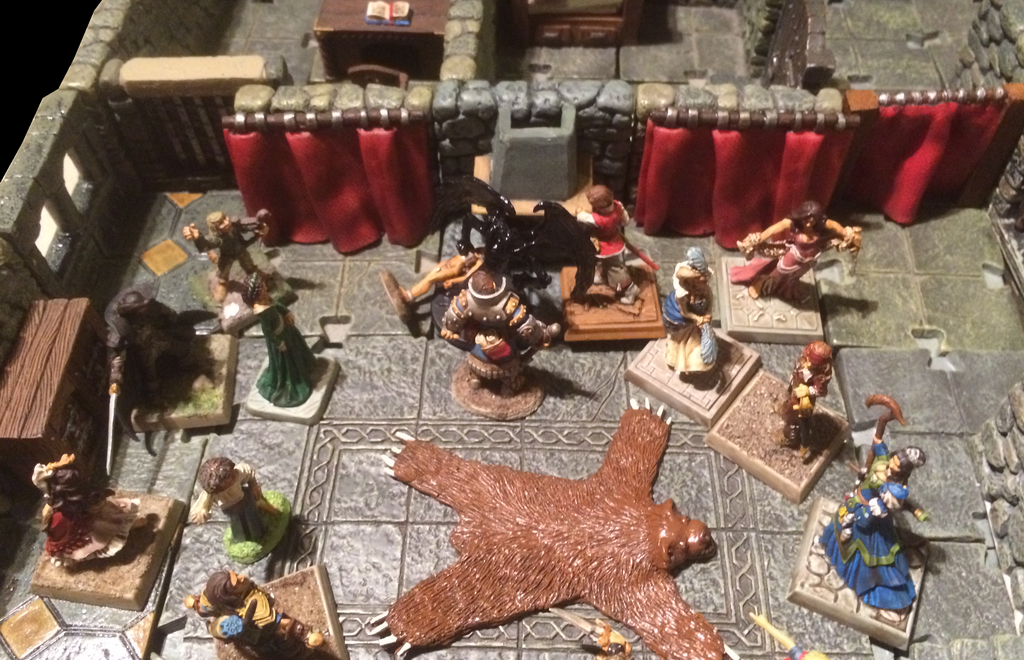
\includegraphics[width=0.39\textwidth]{images/Carowyn-villa-shadow-attack-486296086.jpg}
	\caption{Carowyn villa shadow attack}
	\label{fig:Carowyn-villa-shadow-attack-486296086}
\end{figure}

